\chapter{A Brief Note on Feature Engineering \label{chapter:feateng}}

All machine learning algorithms and statistical models depend on the concept of a \textbf{feature}. A feature is some aspect of a dataset that, the model designer believes, represents the data in a way that is relevant to the problem he/she is trying to solve. 

Before any algorithm can be applied, therefore, it is necessary to decide how to represent the data: which features to include and how to extract them from the raw data. This task is called \textbf{feature engineering}.

%%%%%%%%%%%%%%%%%%%%%%%%%%%%%%%%%%%%%%%%%%%%%%%%%%%%%%%%%%%%%%%%%%%%%%

\section{Study Design vs. Feature Engineering}

We have seen a large number of features in Chapters~\ref{chapter:overview}--\ref{chapter:logreg}, but we never stopped to consider them. That's because, in many datasets, the features are chosen at the \textbf{study design} stage. The analyst (statistician, data scientist, etc.) has no say in what the features look like or which features are included.

This paradigm is changing as data science increasingly focuses on large, observational datasets, like those from electronic medical records (EMRs). In these types of studies, the raw data were not collected for the study itself, but to fulfill some other purpose. The analyst must choose how to build features from the raw data and use them in models.
\vspace{4mm}

\begin{question}{}
The examples in Chapters~\ref{chapter:classification} and~\ref{chapter:regression} used the same two features. What were these features? How were they represented? What are some alternatives to this choice of features?
\end{question}

\begin{question}{}
In Chapter~\ref{chapter:decisiontrees}, we looked at the Wisconsin Breast Cancer Dataset, which includes $30$ different imaging features relevant to predicting whether a tumor is benign or malignant. How were these features represented? What are some alternatives to this choice?
\end{question}

\begin{question}{}
In Chapters~\ref{chapter:linreg} and~\ref{chapter:logreg}, we looked at two datasets that were collected for the purposes of answering particular questions. Do you agree with these study designers' choice of features? What other features could potentially have been relevant to answering each research question?
\end{question}

%%%%%%%%%%%%%%%%%%%%%%%%%%%%%%%%%%%%%%%%%%%%%%%%%%%%%%%%%%%%%%%%%%%%%%

\section{Turning Data into Numbers}

A model is just a tool for learning relationships among sets of numbers. The first step in any data science problem, therefore, is deciding how to represent what is often a large, complex, noisy dataset as a set of numbers. 

\subsection{Numbers}

Sometimes you get lucky and the feature you need is already a number, such as a vital sign measurement, lab value, or other biomarker. In that case, more often than not, the feature enters into the model as its raw value.

In some cases, you may also choose to apply a \textbf{transformation} to the feature before it enters the model. A transformation is simply the application of a deterministic mathematical function that changes the shape of the distribution of the feature. Transformations are often used to improve the interpretability of a model and/or to ensure that the model fulfills the assumptions of the statistical inference method(s) being used (e.g., a hypothesis test).
\vspace{4mm}

\begin{question}{}
Here are $100$ random samples from a normal distribution with $\mu = 3.0$ and $\sigma = 0.5$ and five different transformations of those samples. What do you notice about the shape and position of the data under the different transformations?
\begin{center}
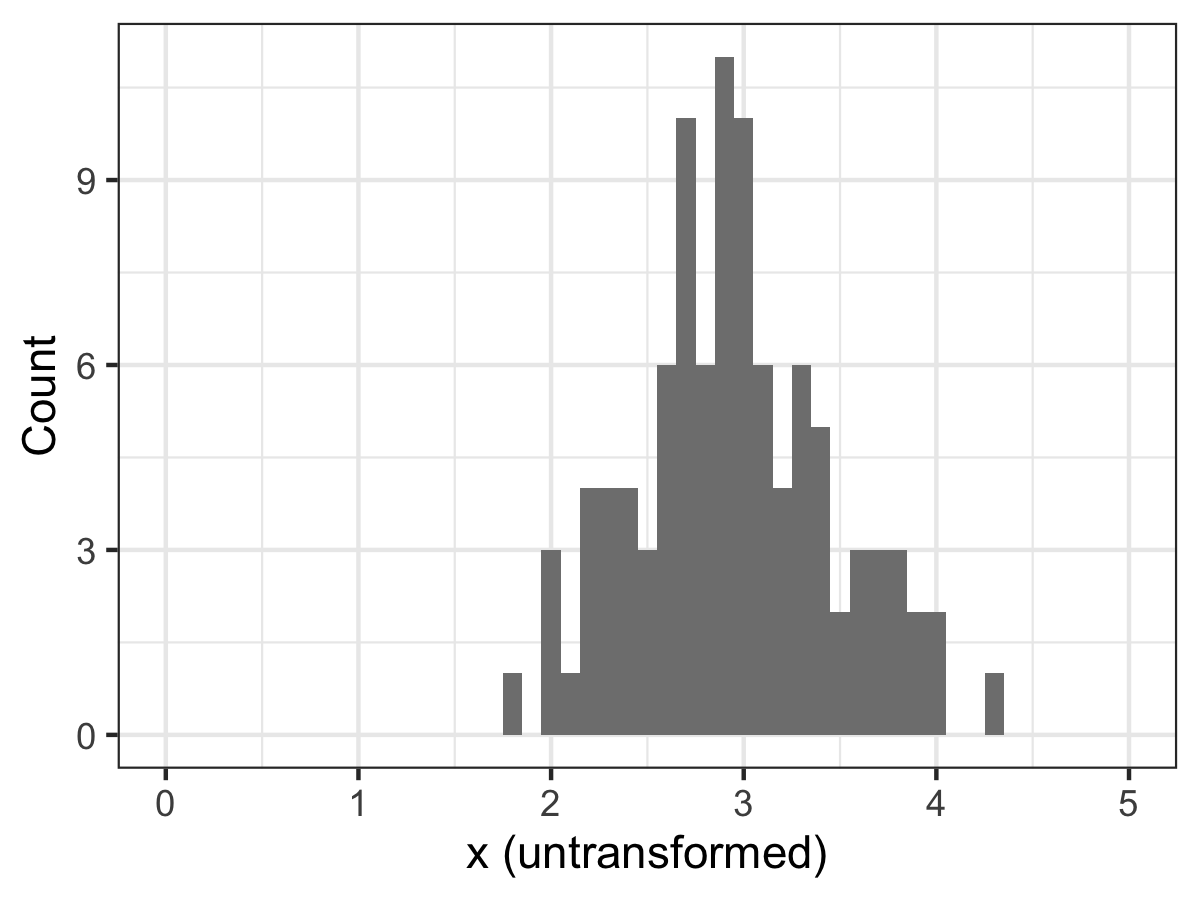
\includegraphics[width=0.4\textwidth]{img/normal-transform-0.png}
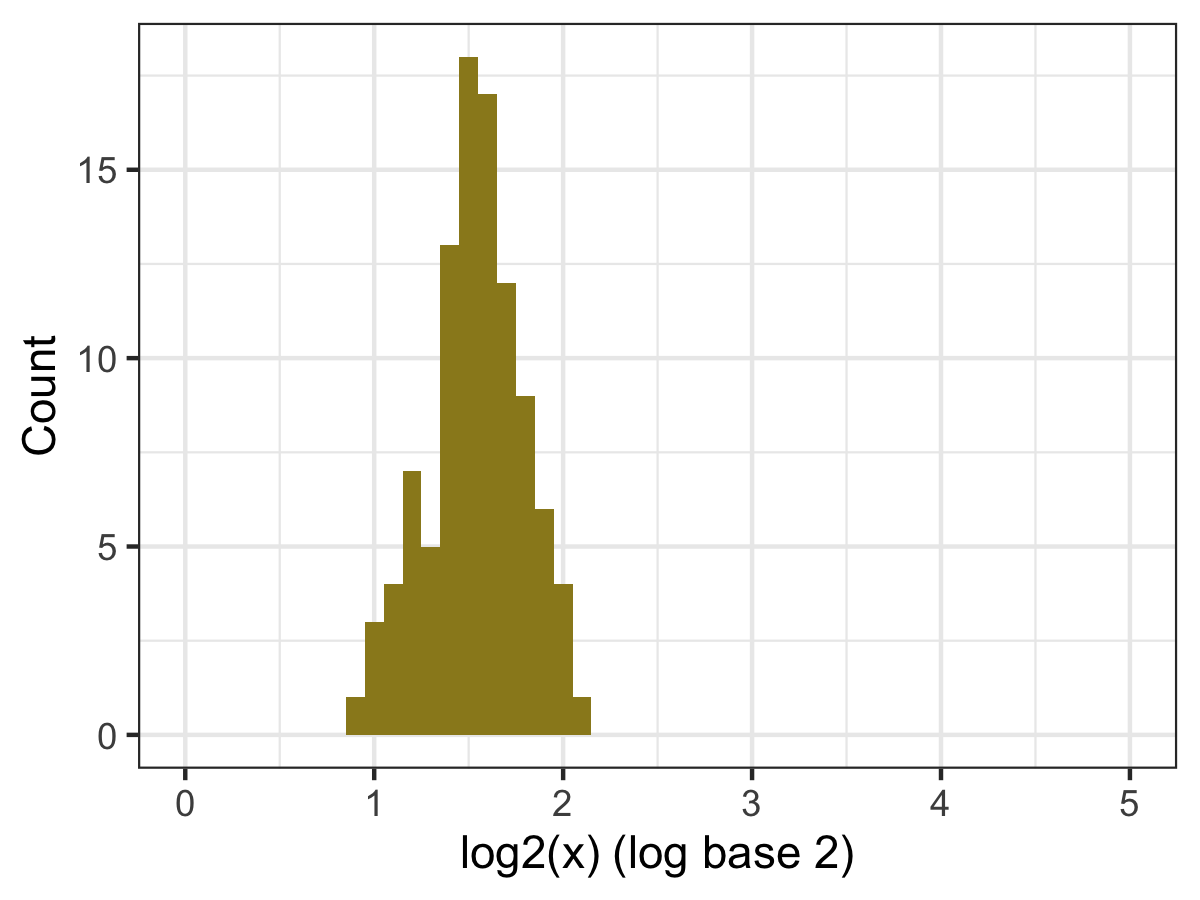
\includegraphics[width=0.4\textwidth]{img/normal-transform-1.png}
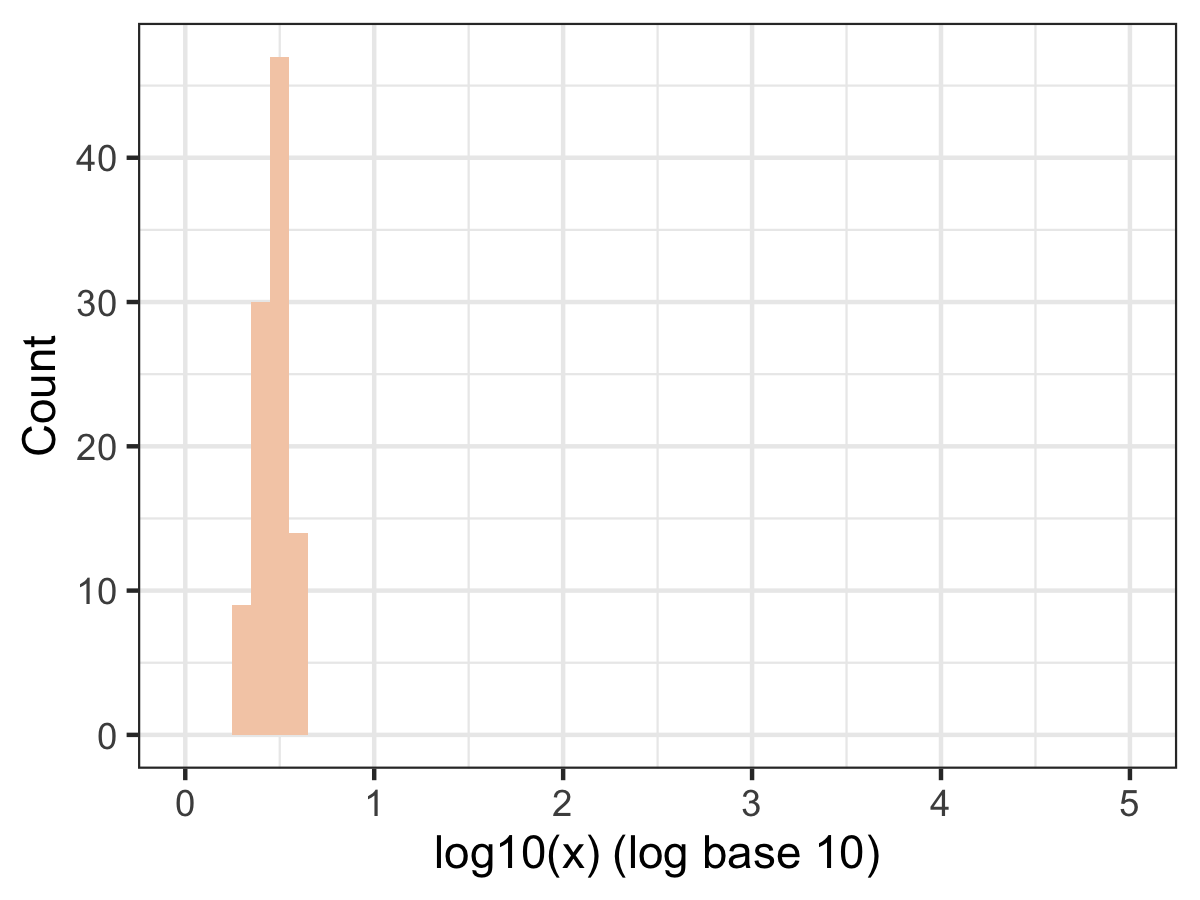
\includegraphics[width=0.4\textwidth]{img/normal-transform-2.png}
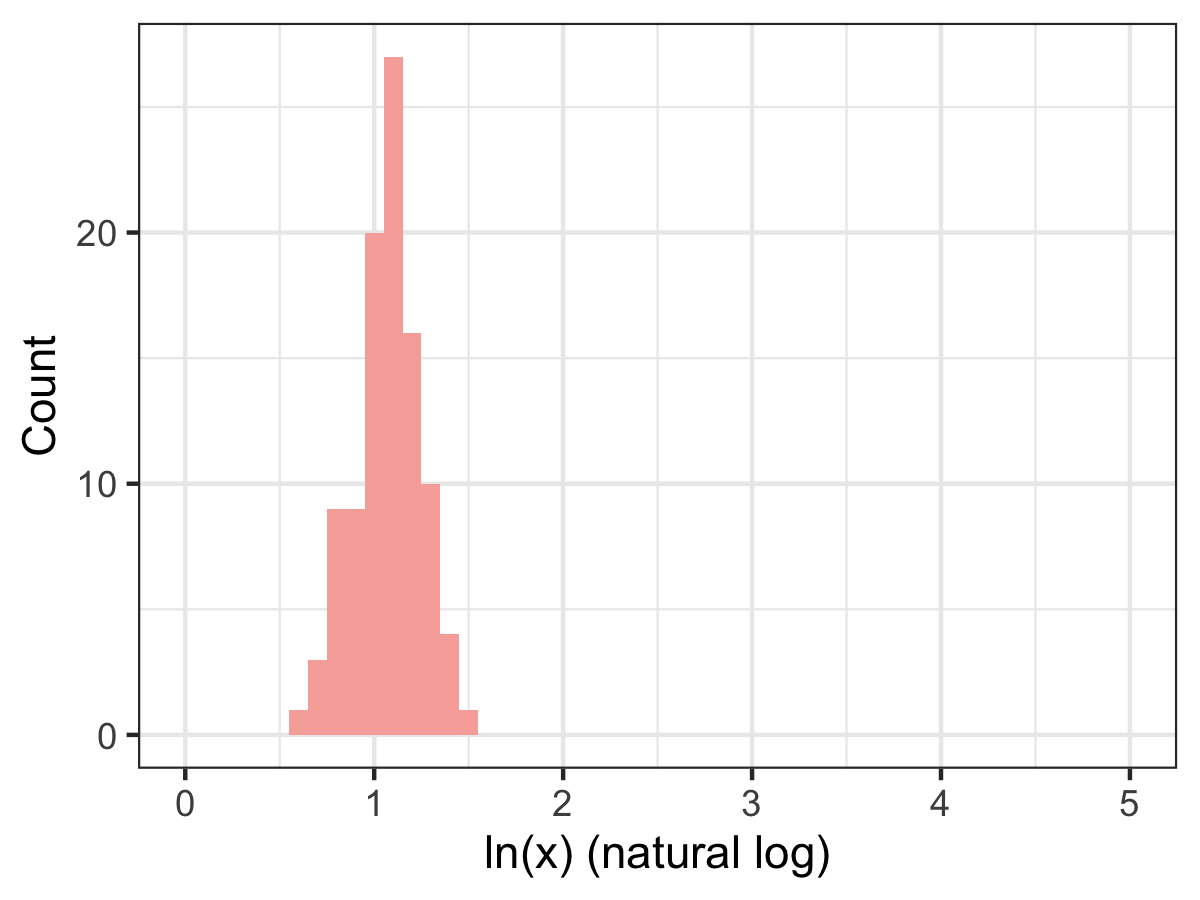
\includegraphics[width=0.4\textwidth]{img/normal-transform-3.png}
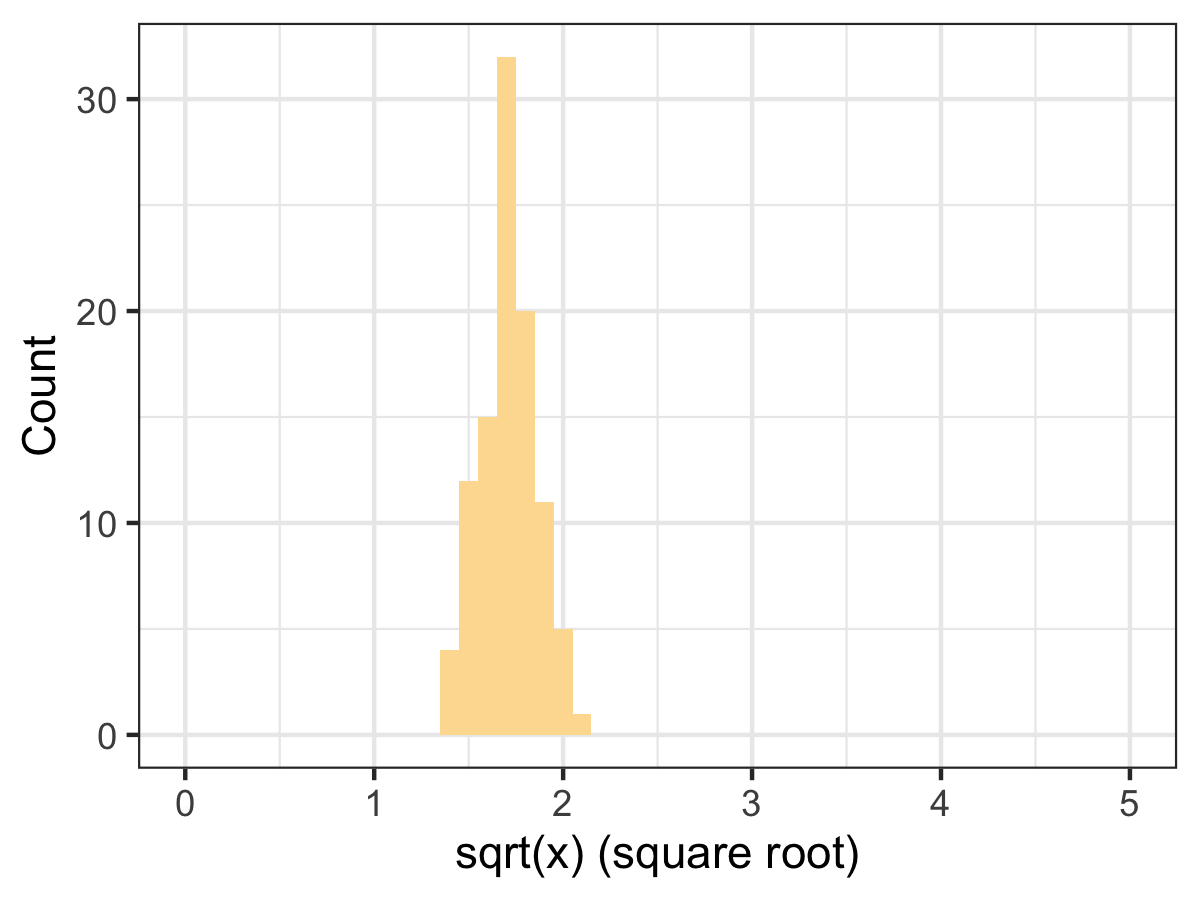
\includegraphics[width=0.4\textwidth]{img/normal-transform-4.png}
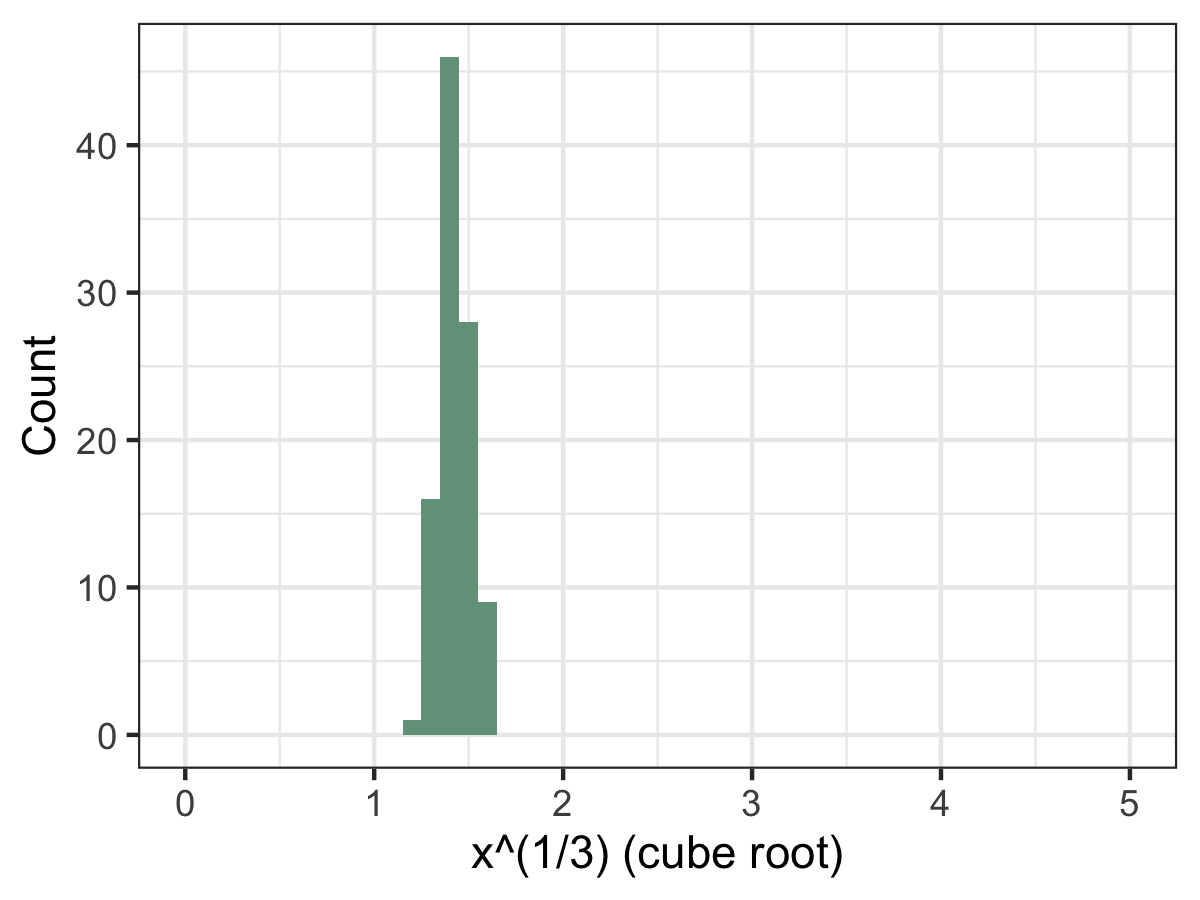
\includegraphics[width=0.4\textwidth]{img/normal-transform-5.png}
\end{center}
\end{question}

\begin{question}{}
Here are $100$ random samples from an exponential (see Section~\ref{sect:exponential}) distribution with $\lambda = 0.8$ and the same five transformations of those samples. What do you notice about the shape and position of the data under the different transformations?
\begin{center}
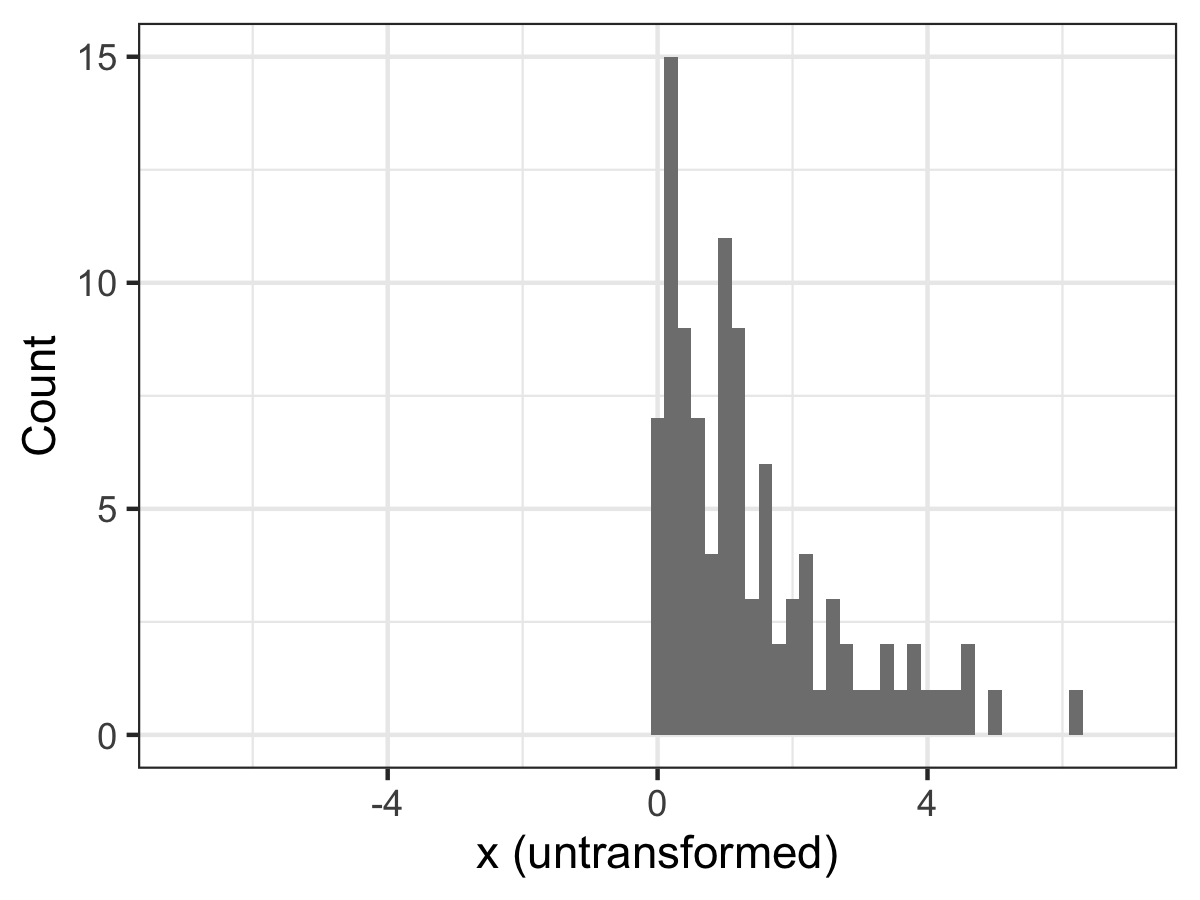
\includegraphics[width=0.4\textwidth]{img/exp-transform-0.png}
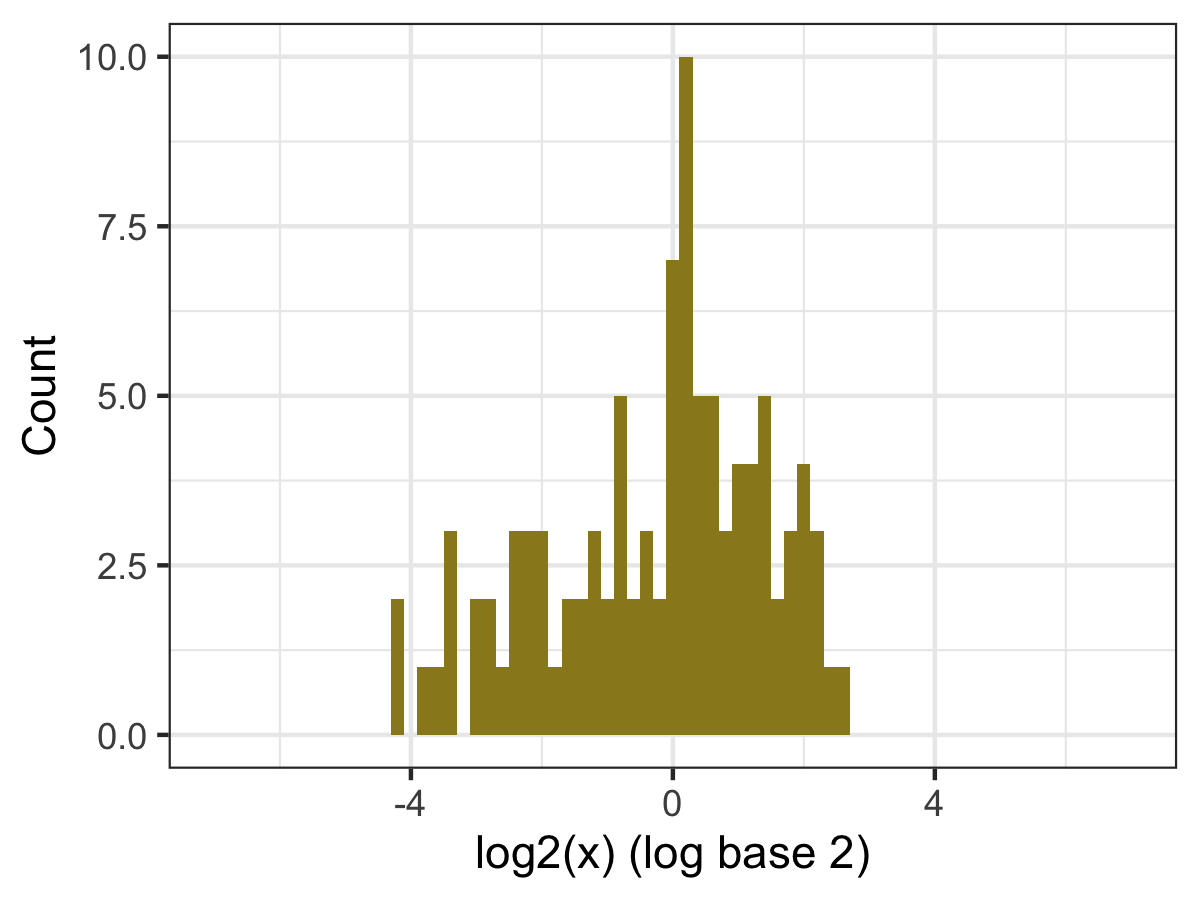
\includegraphics[width=0.4\textwidth]{img/exp-transform-1.png}
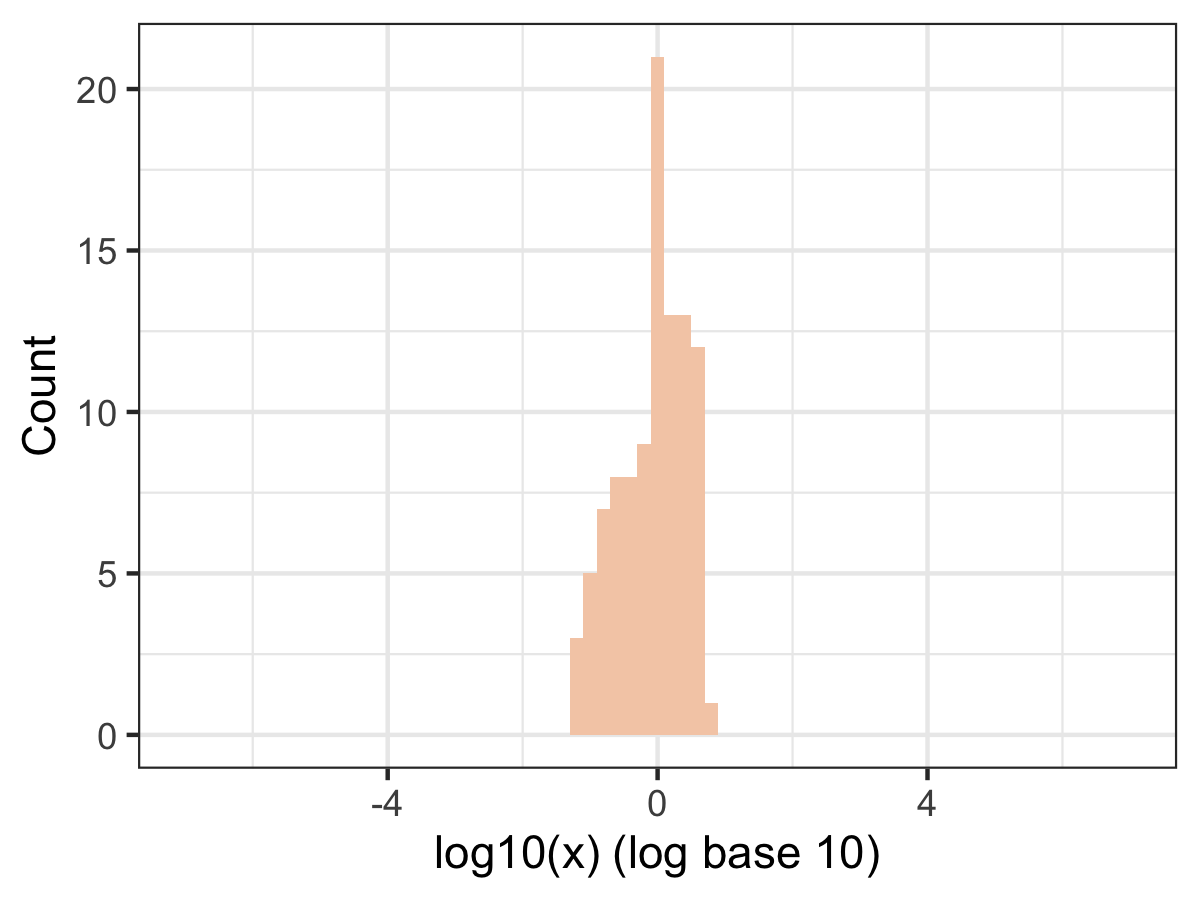
\includegraphics[width=0.4\textwidth]{img/exp-transform-2.png}
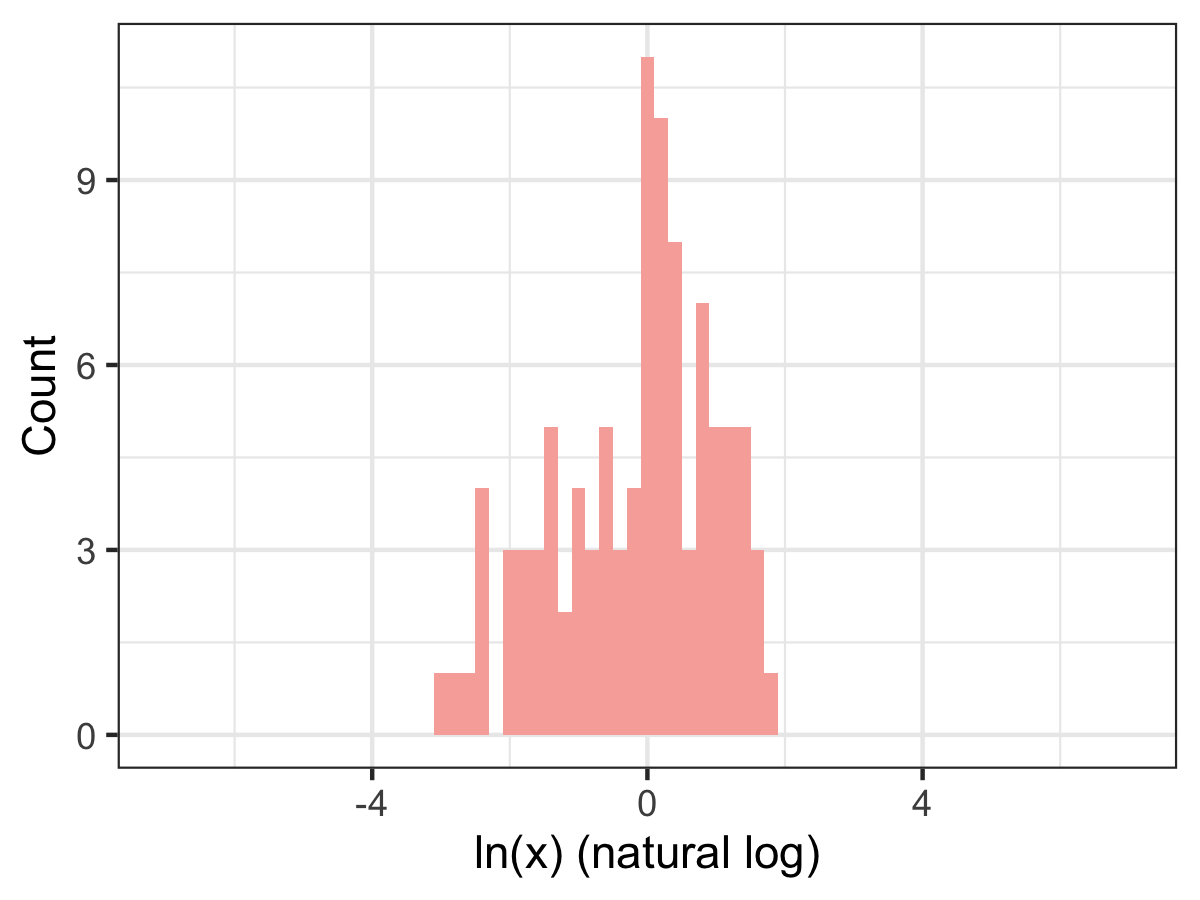
\includegraphics[width=0.4\textwidth]{img/exp-transform-3.png}
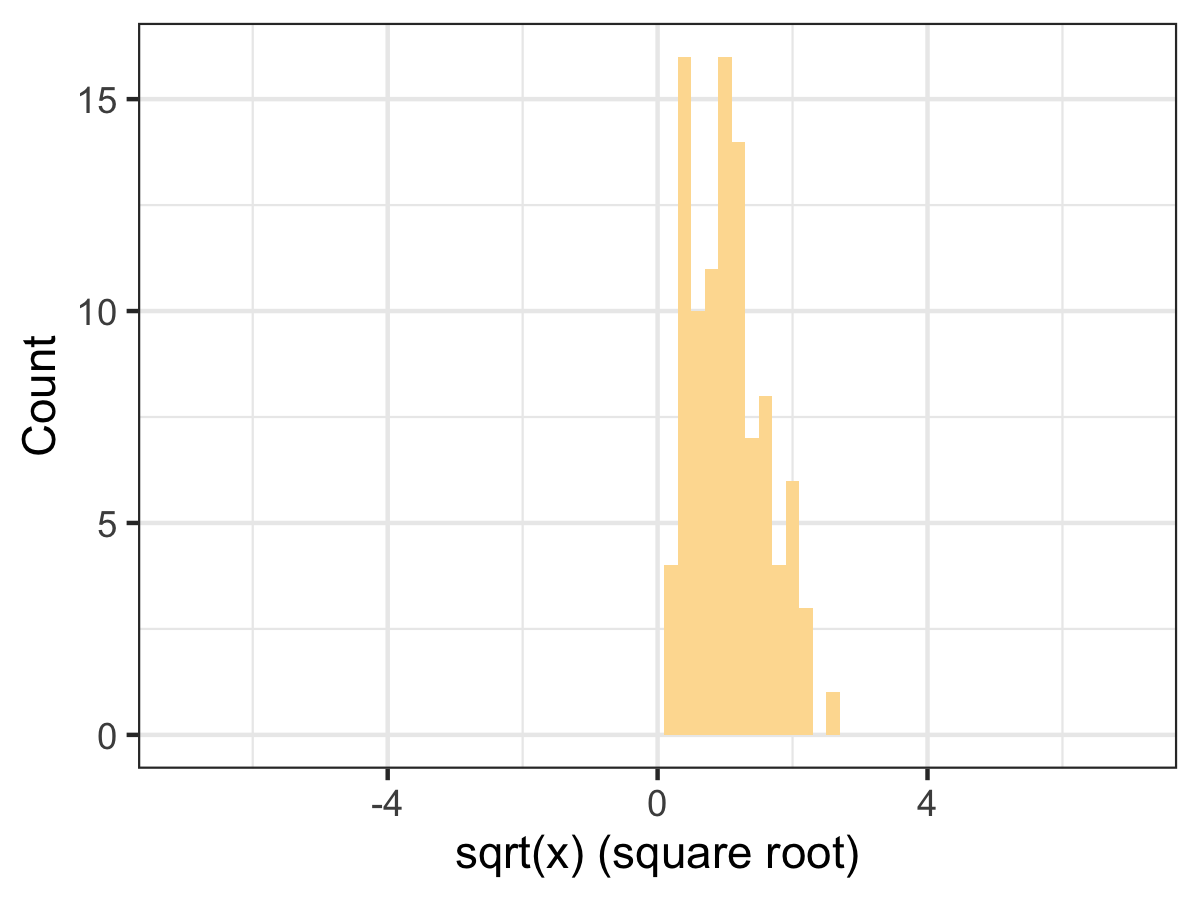
\includegraphics[width=0.4\textwidth]{img/exp-transform-4.png}
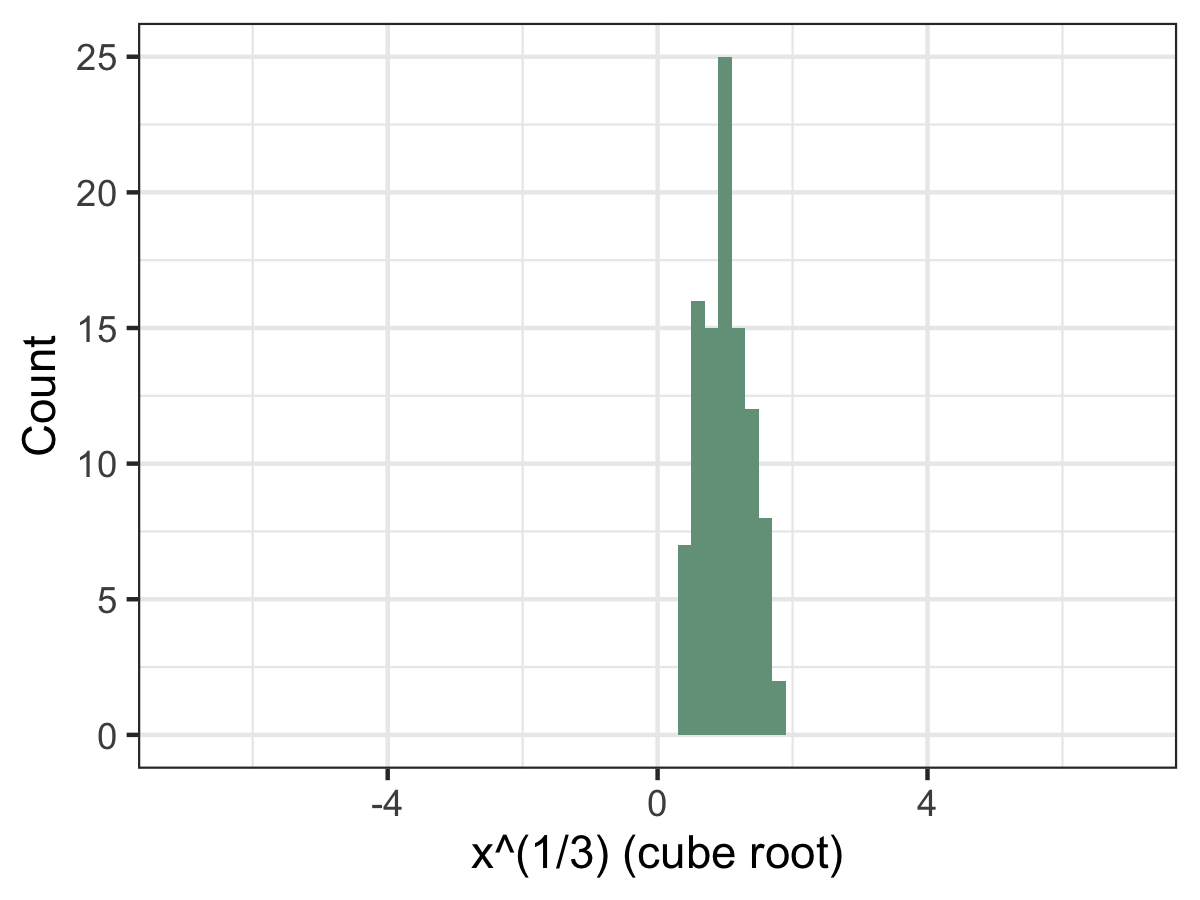
\includegraphics[width=0.4\textwidth]{img/exp-transform-5.png}
\end{center}
\end{question}

Economics, the social sciences, and related disciplines, which are heavily dependent on the use of regression models and hypothesis tests, rely extensively on transformations. In my experience, machine learning folks spend almost no time on them because their primary concern is predictive accuracy, not model interpretation. Machine learning practitioners, however, very frequently \textbf{scale and center} their predictors (see footnote in Section~\ref{section:sehyp}), which is another type of transformation. We will get into more detail on transformations as we continue to learn about regression models. 

\subsection{Binary Variables}

For features which are yes/no (e.g., presence/absence of a disease, symptom, physical attribute, etc.) the most common coding scheme is to use ``1'' for ``yes'' and ``0'' for ``no''. This is useful for interpretation, particularly in regression models. In a linear regression model using this coding scheme, for example, the model coefficient will be the shift in the mean of the normal distribution representing the outcome, $y$, when the feature is present. 

\subsection{Categories}

Categorical features with $k>2$ categories are generally represented using \textbf{indicator variables}. If a feature, $x$, has $k$ \textbf{levels}, we can use $k-1$ yes/no indicator variables to represent that feature. For example, assume $k = 3$ and the possible levels of our feature, $x$, are $A$, $B$, and $C$. We set:
\begin{align*} 
x_1 &= \left\{ \begin{array}{cl} 1 & \text{ if }x = A \\
                                                0 & \text{ otherwise} \end{array} \right. \\[2mm]
x_2 &= \left\{ \begin{array}{cl} 1 & \text{ if }x = B \\
                                                0 & \text{ otherwise} \end{array} \right.
\end{align*}
If the value of $x$ is $A$, $x_1 = 1$ and $x_2 = 0$. If it's $B$, $x_1 = 0$ and $x_2 = 1$. The value $C$ is called our \textbf{reference category} and has $x_1 = 0$ and $x_2 = 0$. In this way, information about all three categories is captured using only two variables. Creating indicator variables is just another way of transforming the value of a feature.
\vspace{4mm}

\begin{question}{}
In Section~\ref{sect:lowbwt}, we saw an example of a model that predicts whether or not a mother will give birth to a low birthweight baby. One of the factors considered in that model is the mother's race, which was coded (crudely and probably inaccurately, I might add) as \texttt{1 = white, 2 = Black, 3 = other}. You can tell how the feature \texttt{RACE} was coded by examining the model output. How many indicator variables were used? Which level of the feature was used as the reference category?
\end{question}



